\section{Graphs of Evaluation Functions} \label{Graphs}

The first natural step was to draw and examine graphs of evaluation functions. One can only draw graphs of functions that contain two or three independent variables. In case of three independent variables, we chose one of the variables (the least significant) as parameter and draw graphs of two remaining variables while changing the parameter\footnote{Therefore the fourth dimension was de facto time.}. 

After constructing and comparing all the graphs, we could say very little about them. We came up with some very obvious results, i.e. that the {\it double founded implication \/} graph equals the {\it founded implication \/} graph when the parameter $c=0$. We also noticed that some graphs looked similar, but still slightly different. These findings do not have formal relevance.

Yet we obtained one interesting result. It is the comparison of the {\it founded equivalence \/}
and {\it pairing \/} quantifiers. The {\it pairing \/} quantifier is defined only by $a$ and
$d$, {\it founded equivalence \/} uses additionally $n$, size of the contingency table. We used
$n$ as parameter for the graph. The two graphs can be seen in figure \ref{fig:FEPairing}.

\begin{figure}[ht]
\centering
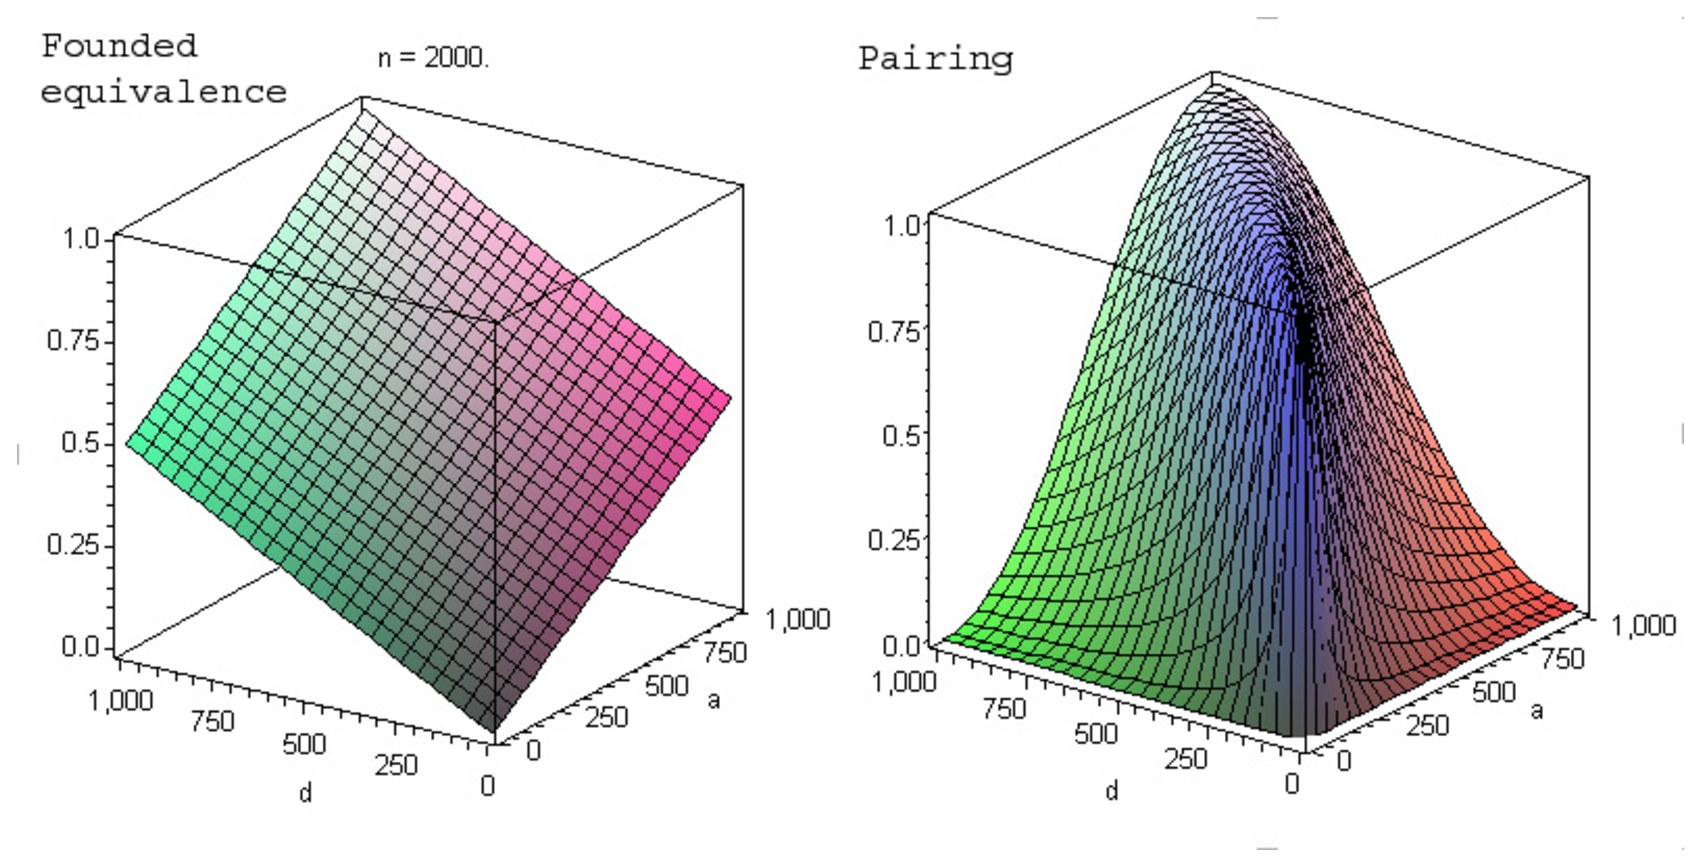
\includegraphics[width=115mm]{FE-Pairing.eps}
%\mbox{\resizebox{125mm}{!}{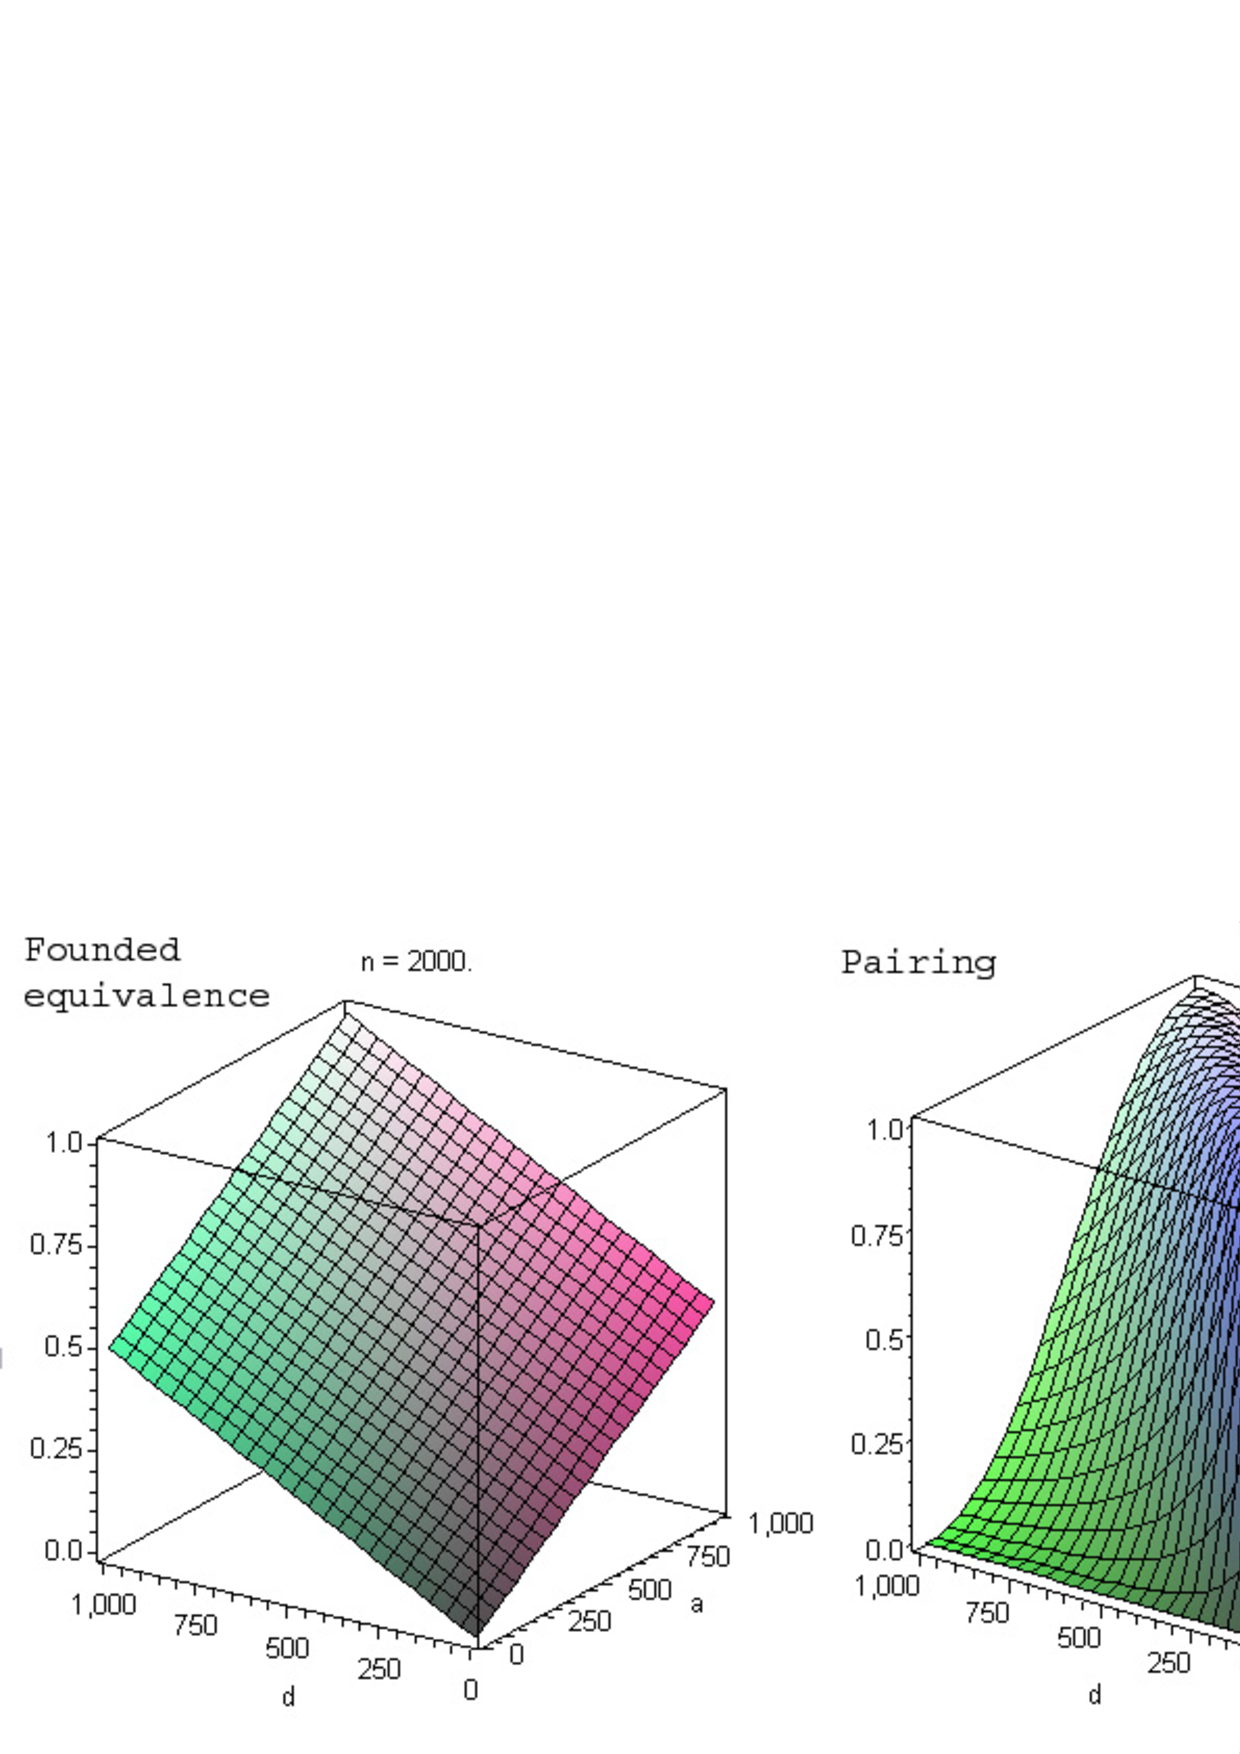
\includegraphics{FE-Pairing.png}}}
\caption{Founded equivalence and Pairing quantifiers graphs}
\label{fig:FEPairing}
\end{figure}

According to \cite{RK:07,Kupka}, the {\it founded equivalence \/} quantifier should be used to find \emph{equivalent occurrence} between $\varphi$ and $\psi$. According to \cite{Kupka} the 
{\it pairing \/} quantifier should search for pairs of \emph{Boolean attributes} that \emph{attract} each other. The two verbal interpretations of the quantifiers are semantically close, one can say that being in pair implies equivalent occurrence, or that equivalent occurrence means being together in one item of the analyzed data, which can be interpreted as being in pair.

To clarify the loose verbal interpretations, we can examine the evaluation functions, which is particularly hard for the {\it pairing \/} quantifier. This is the point where graphical help is necessary. The {\it founded equivalence \/} graph is a plane that increases with $a$ and $d$ and its slope is determined by $n$. Contrary, the {\it pairing \/} quantifier's graph is a "ridge" above the $a d$ diagonal. Then, the characterizing property of the {\it founded equivalence \/} is \emph{the bigger a+d, the better}\footnote{This was apparent also from the evaluation function.} and for {\it pairing \/} quantifier \emph{the more a=d the better}.

Both quantifiers have disadvantages: {\it founded equivalence \/} is unable to distinguish between $a$ and $d$, which is in contrary with the presumption that {\it founded equivalence \/} should be a stronger {\it founded implication \/}. The {\it pairing \/} quantifier on the other hand is unable to consider $b$ and $c$, thus resulting rule may be weakly supported. 

The analysis shows us how to use both quantifiers in a more profound way. When using {\it founded equivalence \/}, we should also look at the ratio of $a/d$ to see how good the rule is in terms of positive and negative examples. We should use {\it pairing \/} quantifier to find balanced all-positive, all-negative examples ratio; it is preferable to aid
with the {\it founded equivalence \/} evaluation function. This new perception of the two quantifiers was made possible mainly by examining their graphs.

\medskip

One of the initial motivations was to examine, how does the \emph{founded implication}
correlate with \emph{lower critical implication }and \emph{upper critical implication}.
The only way to graph critical implications is to set $p$ as parameter, which
makes them incomparable to the \emph{founded implication}, where the $p$ is value
of two-dimensional function. This problem is solved in section \ref{Graphs_Tables} by
displaying graphs of critical frequencies of quantifiers. 